\section{Introduction}
\label{introduction}

%Here is a problem
Upcoming memory technologies, such as Intel/Micron's recently-announced 3D XPoint
memory~\cite{3dcrosspoint}, are projected to be denser and cheaper per bit than DRAM while
providing the byte-addressable load-store interface of conventional main memory.
Improved capacity and cost per bit come at the price of higher access latency,
projected to fall somewhere in the range of 400ns to several
microseconds~\cite{3dcrosspoint} as opposed to $\approx$ 50--100ns for DRAM. The impending commercial availability of such
devices has renewed interest in two-tiered physical memory, wherein part of a
system's physical address space is implemented with the slower, cheaper memory
technology~\cite{ref:Dulloor:datatiering,qureshi:twolm}.  Slow memory can result in a net cost win if the cost savings of
replaced DRAM outweigh cost increase due to reduced program performance or by
enabling a higher peak memory capacity per server than is economically viable
with DRAM alone. For a 50\% occupied data center the capital expenditure is
estimated to be 17\%\cite{borosso2013}. If we assume that slow memory is 1/3 as cheap as
DRAM and that main memory is 30\% of the machine cost, then the maximum
cost that can be saved from deploying such memory technology is 3\%. For this reason, we set tolerable performance
degradation to at most 3\% of the performance of a DRAM-only system in this study.

%This is of especial interest to cloud service providers since
%DRAM costs are a significant part of overall data center total cost of ownership
%(TCO).
%Figure~\ref{fig:motivation} shows that over half of the memory
%footprint (when allocated in 4KB pages) of representative cloud applications are
%identified as idle/cold by Linux's {\tt kstaled} mechanism (an optional extension to
%the Linux kernel that tracks pages that have not been Accessed over a fixed time
%interval)~\cite{kstaled}, indicating that the corresponding pages have an
%inter-access interval exceeding 20s. 
%%\todo{Analytic modeling (discussed in
%%Section~\ref{analytic-model}) suggests these pages could be shifted to a memory
%%with a 3us access time with negligible (<3\%) performance degradation.}
%
\begin{figure}[t]
\centering
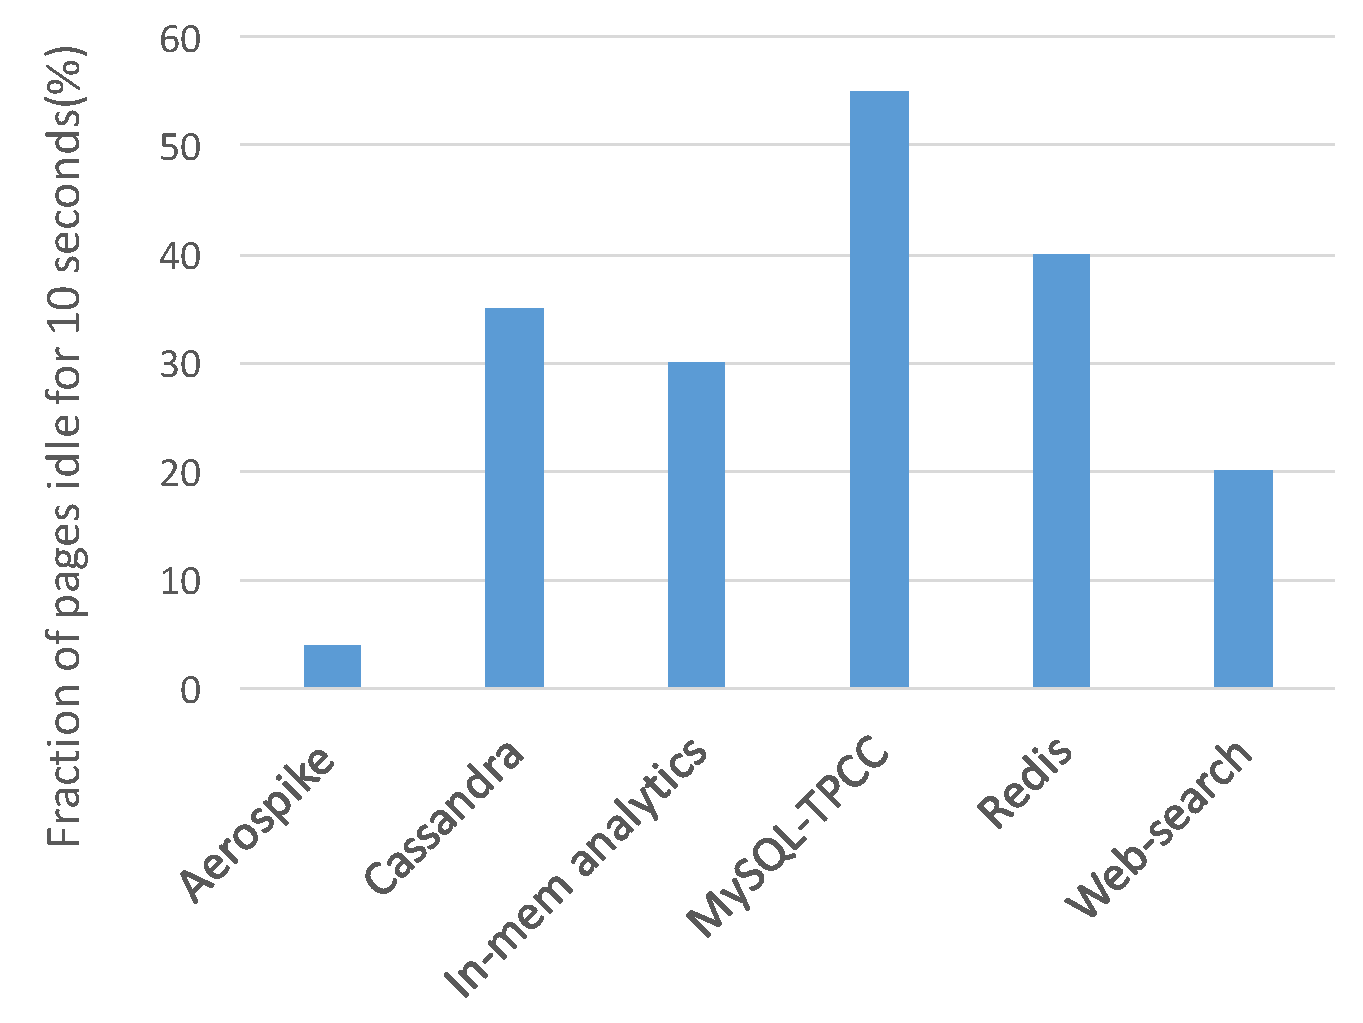
\includegraphics[width=1.0\columnwidth]{asplos2017/figures/kstaled-cold-data-10s}
\caption{Amount of 2MB pages idle for 10sec detected by per-page {\it Accessed} bit
in hardware. Note that this technique cannot estimate the page access rate, and
is thus incapable of estimating the performance degradation caused by placing
these pages in slow memory (in fact the performance degradation can be greater
than 10\% for Redis).}
\label{fig:motivation}
%\vspace{-0.225in}
\end{figure}

%It's an interesting problem
However, deploying such memories by a cloud service provider for use by its
customers is riddled with several problems. It is important for cloud providers
to be able to provide service-level-agreements (SLAs) to customers about
performance of the cloud platform. To provide such SLAs in the presence of slow
memory, any memory placement policy must estimate the performance degradation
associated with placing a given memory page in slow memory, which in turn requires some
method to gauge the {\it page access rate}. Lack of accurate page access
rate tracking in contemporary x86 hardware makes this task challenging.
Moreover, as we will show, naive policies to place pages into slow memory based
on existing hardware-maintained {\it Accessed} bits are insufficient and can lead to severe
performance degradations, which can result in broken SLAs.
%on their estimated access frequency can lead to severe performance degradations
%which can result in broken SLAs.

Making slow memory usage application transparent is particularly
critical for cloud computing environments, where the cloud provider may wish to
transparently substitute cheap memory for DRAM to reduce provisioning cost, but
has limited visibility and control of customer applications.  Relatively few
cloud customers are likely to take advantage of cheaper-but-slower memory
technology if they must redesign their applications to explicitly allocate and
manage hot and cold memory footprints. A host-OS-based cold memory detection and
placement mechanism is a natural candidate for such a system.
Figure~\ref{fig:motivation} shows the amount of data idle for 10s as detected at
runtime by an OS-based hardware {\it Accessed} bit monitoring technique for various
cloud applications. We observe that substantial cold data (more
than 50\% for MySQL) can be detected by application-transparent mechanisms.

However, there has been little work on providing performance degradation
guarantees in the presence of page migration to slow
memory~\cite{li2015managing}. 
Furthermore, prior work on two-tiered memory has assumed migration/paging at 4KB
page granularity~\cite{qureshi:twolm,ref:Dulloor:datatiering}. However,
huge pages (2MB pages) are now ubiquitous and critical, especially for cloud
platforms where virtualization magnifies the costs of managing 4KB pages.
We observe a performance improvement that is as high as 30\% from huge pages under
virtualization (Table~\ref{tab:thp-benefit}).
Our proposal, {\it Thermostat}, manages two-tiered main memory
transparently to applications while preserving the benefits of huge pages 
and dynamically enforcing limits on performance degradation (e.g., limiting 
slowdown to 3\%).
 In Section~\ref{proposal} we show that Thermostat is huge-page-aware and can
place/migrate pages at huge page granularity with a minimal overhead, and
furthermore satisfies performance degradation guarantees, thereby meeting SLAs.
%Indeed, huge pages are so performance critical that some cloud vendors report
%mapping {\tt temps} file systems to huge pages as
%well~\cite{Linux-mailing-list} \fixme{it's not obvious to me why tmpfs is
%important.  The implications of this sentence need to be clarified}.
%Table~\ref{tab:thp-benefit} demonstrates the criticality of 2MB huge pages under
%virtualization. We see as much as 30\% performance improvement from huge pages.
%As we shall see in Section~\ref{XXX}, Thermostat has been designed keeping
%hugepages in mind.

%It's an unsolved problem
Prior work has considered two approaches to two-tiered memory: (i) a paging
mechanism~\cite{Lim2012,Lim2009}, wherein accesses to slow memory invoke a page
fault that must transfer data to fast memory before an access may proceed, and,
(ii)
via a migration mechanism (as in cache coherent NUMA
multiprocessors)~\cite{AUTONUMA}, wherein no software fault is required.  In the
latter scenario, a migration mechanism seeks to shuffle pages between tiers to
maximize fast-memory accesses. Dulloor et al.~\cite{ref:Dulloor:datatiering}
have described a programmer-guided data placement scheme in NVRAM. Such
techniques are impractical in many cases like closed-source database engines,
where the source code for customer applications are unavailable to the customers
themselves. Li et al.~\cite{li2015managing} describe a
hardware-based technique to accurately gauge the impact of moving a page from
NVRAM to DRAM. However, such hardware requires significant changes to
contemporary x86 architecture. Requiring extra architectural changes to an
established platform such as x86 will only delay the adoption of a technique
due to the long lead-time in ordering and installation of custom components. We
do not require {\it any} extra hardware changes apart from the availability of a
slow memory interface, which makes our technique easily applicable to any
architecture with such support.

To design a low overhead cold page detection mechanism Thermostat continuously samples a
small fraction of pages and estimates page access rate by spatial extrapolation
(described in Section~\ref{page-sampling}).
This strategy makes Thermostat both low overhead and fast-reacting. The single
\emph{Accessed} bit per page provided by hardware is insufficient to distinguish hot
and cold pages with sufficiently low overhead.  Instead, Thermostat uses TLB misses as a proxy for LLC misses 
as they can be tracked in the OS through reserved bits in the PTE, allowing page access rates to be estimated at low overhead.
%We see that for high-memory-footprint applications, TLB misses and LLC misses are
%within a factor of two, with TLB misses being typically higher than LLC misses.  
Finally, Thermostat employs a correction mechanism that rapidly detects
and corrects mis-classified cold pages (e.g., due to time-changing access patterns).

%To achieve this goal, we employ three techniques.
%a) {\it Leveraging spatial locality for low overhead sampling:} Simply poisoning
%a fraction of application pages is either too high overhead (due to poisoning a
%high number of pages) or too slow-reacting (due to only poisoning a small
%fraction of application pages). We solve this dilemma by relying on the spatial
%locality of memory accesses, i.e., access frequencies of nearby memory locations
%are similar. Using this property, we only profile a small fraction of pages, and
%deduce the access frequency of other pages based on the access frequencies of
%the profiled pages. In Figure~\ref{nocorrections} we can see that by profiling
%only a small fraction of pages, we can reduce the profiling overhead to be
%negligible (XXX\%). However, when using such estimates in Thermostat, the
%performance degradation can be seen to be much higher than what is targeted
%(XXX\% as opposed to XXX\% targeted).
%
%b) {\it TLB miss based page access estimates:} Current x86 hardware does not
%support tracking page accesses at a page level granularity. A sample of accesses
%can be collected by PEBS, but this technique needs to be run at a very low
%sampling rate (< 1000 samples/s per recommendations on perf
%website~\cite{perf-website}) for it to be low overhead. To overcome this
%difficulty, we use BadgerTrap~\cite{badgertrap}, which is a kernel based
%mechanism to poison arbitrary pages and thereby observe all TLB misses to those
%pages. In cloud workloads, TLB misses can be fairly closely correlated with LLC
%misses (shown in Section~\cite{tlb-vs-llc}) and thus this is a viable technique
%to get good estimates of number of accesses to different pages. In
%Figure~\ref{allhugepages} we show the performance degradation in Redis caused by
%a policy that poisons 5\% of all pages for profiling. As we can see, Redis
%throughput is severely degraded (XXX\%) by such a system.
%
%c) {\it Correcting wrongly placed pages:} With any policy, there are always
%bound to be some mis-classified pages: either due to the mistakes made by the
%policy or due to the time-changing access pattern of the workload. We thus track
%the actual page access frequency and compare it to the expected page access
%frequency, and revert decisions that are deemed to be incorrect (described in
%Section~\ref{XXX}). In Figure~\ref{finalpolicy} we can see that by using our
%correction mechanism the policy correctly keeps performance degradation under
%the targeted amount, and also places significant amount of data in slow memory.

%Huge pages thwart prior two-tiered memory proposals because it is difficult
%to determine the access rate of a 2MB huge page at low overhead. OS-based idle 
%page tracking mechanisms, such as {\tt kstaled}, periodically scan and 
%reset the ``Accessed'' bit in the page table entry for a page.
%This bit is set by the hardware page walker each time a TLB miss
%accesses the page. However, such coarse grained access information is difficult
%to use for estimating performance slowdown. To estimate the performance slowdown
%when a page is placed in slow memory, Thermostat needs to estimate the page
%access frequency of that page (under the assumption that performance slowdown is
%approximately proportional to the rate of access to slow memory).

%The single ``Accessed'' bit per 2MB page, scanned at 20s granularity, provides insufficient
%information to classify a large fraction of 2MB pages as cold. 
%As shown in Figure~\ref{fig:motivation}, such a straight-forward extension of
%{\tt kstaled} identifies only a small fraction of 2MB pages as idle/cold---far less than
%the 50\% fraction of cold memory footprint identified when scans are performed at 4KB granularity.
%Simply splitting all huge pages, however, abandons the substantial (8-30\%) performance 
%boost provided by the transparent huge-page mechanism.  These observations 
%motivate a redesign of the idle/cold page detection mechanism to be aware of
%huge pages and identify both 2MB and 4KB pages that can be profitably
%migrated to slow, cheap memory.
%it is too expensive to frequently migrate pages at 2MB granularity. \todo{Neha:
%What is the expense here? If the same amount of cold data is being transferred
%it should take approximately the same time regardless of 4KB or 2MB pages (2MB
%pages might be somewhat faster due to bulk transfers)} \fixme{I think the point
%you want to make is that there is no opportunity to migrate at 2MB, either
%slowdown is too high or too few pages are cold.  Alternatively, if we use only
%4KB pages, we leave the 30\% boost of huge pages on the table.  The point that
%migration is too expensive at 2MB granularity is spurious and shouldn't be said
%here.}

%These hot regions within a huge pages present a central challenge to our
%objective of placing as much data in cheaper but slower memory technology. Since
%prior approaches categorize pages as cold or hot at page granularity, if any of
%the 4KB regions within a 2MB huge page is hot, the entire 2MB page is considered
%to be hot, leading to a significant decrease in the fraction of cold pages. We
%call such pages ``hotspot'' pages.  Figure~\ref{fig:motivation} shows that such
%hotspot pages reduce the fraction of cold data by $\approx$ 50\% when using 2MB
%pages instead of 4KB pages.

%Hotspot pages cause problems in (1) detecting cold pages
%and (2) placing cold pages in slow memory.
%First, since current
%cold page detection mechanisms (e.g., kstaled) in Linux operate by detecting
%accesses at page granularity, \fixme{bad grammar; also repeats points that have already been made: hotspot pages cause very little amount of cold
%data detected by such mechanisms when applied on 2MB pages}. Second, placing the
%hotspot page as a monolithic 2MB page in slow memory causes throughput degradation,
%since the accesses to the hot 4KB regions within that hotspot page are also slowed
%down. \fixme{The second half of this paragraph should be simplified.  It seems repetitive and overly complicated.}
%\begin{table}[t]
%\begin{center}
%\begin{tabular}{|c|c|c|}
%\hline
%&DRAM& NVRAM \\
%\hline
%Read Latency & 100ns  & 200-400ns \\
%\hline
%Cost & 1$\times$ & $\frac{1}{5}\times$ \\
%\hline
%Capacity & 100s of GBs & Terabytes \\
%\hline
%\end{tabular}
%\vspace{0.05in}
%\caption{Comparison of new memory technologies. NVRAM is projected to be cheaper but slower than
%commodity DRAM~\cite{ref:Dulloor:datatiering}.}
%\label{tab:dram-nvram}
%\end{center}
%\end{table}

%Why OS-based design

\begin{table}[t]
\begin{center}
\begin{tabular}{|c|c|}
\hline
&Performance gain\\
\hline
Aerospike&6\%\\
\hline
Cassandra&13\% \\
\hline
In-memory Analytics&8\% \\
\hline
MySQL-TPCC&8\% \\
\hline
Redis&30\%\\
\hline
Web-search&No difference\\
\hline
\end{tabular}
\caption{Throughput gain from 2MB huge pages under virtualization relative to
4KB pages on both host and guest.}
\label{tab:thp-benefit}
\end{center}
\end{table}

%In this work, we present \emph{Thermostat}, a host OS mechanism that can 
%automatically classify both 4KB and 2MB pages as hot or cold at runtime with
%negligible overhead.  Thermostat then uses this classification to migrate
%cold pages to slow, cheap memory while limiting performance degradation to
%3-10\%. 
We implement Thermostat in Linux kernel version 4.5 and evaluate its effectiveness on
representative cloud computing workloads running under KVM virtualization. 
As the cheaper memory technologies we target, such as 3D XPoint, are not yet commercially
available, our evaluation emulates slow memory using a software technique that triggers
translation faults for slow memory pages, yielding a 1us average
access latency.
%We demonstrate that Thermostat can migrate upto 50\% of application memory
%footprint to slow memory while limiting performance
%degradation to 3\%, thereby reducing memory cost upto 30\%.

%%Translation Facades
%To solve this problem, we propose translation facades, a 4KB translation that
%remaps a portion of a 2MB mapping with an alternate physical address. Current
%x86 architecture requires non-overlapping mappings due to hard-coded page table
%structure. However, using translation facades, cold parts of hotspot 2MB pages
%can be placed in slow memory with a single huge page mapping, and the hot 4KB
%pages in the hotspot page can be placed in fast memory by having a 4KB facade
%for each such page. \todo{Neha: How about simply breaking up the hotspot pages
%w/o any facades? Compare against that.}

%Here is my idea
In summary, we make the following contributions: 
\begin{itemize}
%\item We measure hot
%and cold memory fractions at 4KB granularity and within 2MB huge pages to
%measure two-tiered memory opportunity. We use {\tt kstaled}  and
%BadgerTrap~\cite{ref:badgertrap} (a tool to inject soft page faults) to facilitate this
%characterization
\item We propose an online low-overhead mechanism for
estimating the performance degradation due to placing a particular page
in slow memory.
\item We use this mechanism in an online, huge-page-aware hot/cold page
classification system that {\it only} requires a target maximum slowdown
as input.
\item We propose an online method to detect mis-classifications and rectify them,
thereby minimizing the impact of such mis-classifications on application
throughput.
\item By emulating slow memory in software, we demonstrate that Thermostat can
migrate up to 50\% of cloud application footprints to slow memory with
a 3\% slowdown, reducing memory provisioning cost up to 30\%.
\end{itemize}

%We show that using Thermostat, $\approx$ XXX\% of data
%can be placed in slow memory as opposed to only XXX\% when using only 2MB pages.
%We show that placing this cold data in slow memory  leads to a $\approx$ XXX\%
%reduction in workload performance while running under KVM in Linux.

%\item We develop translation facades (using BadgerTrap to emulate
%performance) and investigate novel page table and TLB organizations to support
%facades. We show that using translation facades, $\approx$ XXX\% of data can be placed in slow memory as opposed to only XXX\% when using only 2MB pages. We show that placing this cold data in slow memory only leads to a $\approx$ XXX\% reduction in workload performance while running under KVM in Linux.

%TODO My idea works
%TODO Here's how my idea compares to other people's approaches

%OLD TEXT
%
%Upcoming memory technologies such as Intel 3D-XPoint~\cite{XXX} are an
%attractive candidate for reducing main memory costs (both in terms of CapEx and
%OpEx) in datacenters, which is pegged at 30\% of TCO by recent
%estimates~\cite{XXX}. Such memory technologies have two defining characteristics
%that set them apart from commodity DRAMs: a) they are much cheaper per unit
%capacity than DRAM, with current estimates putting them at $50\%$ cheaper
%than DRAM, and, b) they are much slower than DRAM technology. Whereas
%commodity DDR3/DDR4 has a latency of $\approx$100ns, such upcoming memory
%technologies have latencies of the order of 400ns--1us.
%
%Because of such high access latencies of newer memory technologies, they can
%not completely substitute DRAMs. Instead, a prime area for such
%technologies is for storing {\it cold} data of applications. It has been shown
%that a major fraction (XXX\% by some estimates~\cite{XXX}) of application
%footprint in current cloud/datacenter workloads is {\it cold}, i.e., rarely
%touched by the application. Placing such data in slow memories does not
%degrade the application throughput or latency significantly, while also reducing
%the amount of costly DRAM required in datacenters by a significant margin. In
%order to perform such placement in a application-transparent fashion, the
%identification of cold data is done at an OS page granularity, where a page is
%deemed to be a ``hot page'' if any of the data present in that page is hot.

%As a consequence of this mechanism, when going to larger page sizes (2MB/1GB
%instead of the currently prevailing 4KB), a significantly smaller fraction of
%pages is classified as ``cold''. This is because the presence of even a {\it
%single} hot data item in an otherwise cold page will result in the entire page
%being classified as hot. Using a smaller page size could have identified the
%locations of the hot data more precisely, and thereby resulted in a larger
%fraction of cold pages. Such a ``spotty'' distribution of hot data is common in
%datacenter applications, and according to our estimates, using 2MB sized pages
%reduces the fraction of cold pages by $\approx$XXX$\times$. Thus, using larger
%page sizes cause sub-optimal usage of cheap memory technologies in datacenters.
%
%However, usage of large page sizes, typically done in Linux through {\it
%Transparent Huge Pages (THP)}, is ubiquitous in modern datacenter applications.
%THP is a mechanism available in the Linux kernel whereby
%applications can transparently use large (2MB) or huge (1GB) sized pages without
%any source code change. Larger page sizes has been shown to reduce page faults
%and thereby improve throughput and latency in datacenter applications
%significantly.  Thus, most of such applications are currently run with THP, and
%turning off THP is not a viable solution in most-if-not-all cases. Thus, there
%is a dilemma between choosing THP, thereby benefiting from the large
%application speedups, and not choosing THP, thereby lowering datacenter TCO by
%placing larger fractions of application footprint in cheap memories.
